\section{Design Entry CIS} \label{sec:cis}



%%------- Файл настроек Capture.ini
\subsection{Настройка} \label{ssec:cis_setup}


%%%------- Файл настроек Capture.ini
\subsubsection{Файл настроек Capture.ini} \label{sssec:cis_setup_capture_ini}

В~версии~\textbf{16.6} при~загрузке \textbf{Design Entry CIS} в~консоли выводится путь к~этому файлу. В~\textbf{16.5} "--- лежит в~\textit{<<../SPB\_16.5/tools/capture/>>}. 

Для~корректной работы \textbf{БД} необходимо заполнить в~файле настроек \textbf{Captrue.ini} параметры приведенные в~таблице~\ref{tab:capture_ini}.

\begin{tabularx}{\linewidth}{| m{6.5cm} | X |}
	\caption{Параметры \textit{Capture.ini}} \label{tab:capture_ini} \\
	\hline	
	\calign{Название} 		& \calign{Описание} 					\\ \hline
	\endfirsthead
	
	\multicolumn{2}{r}{продолжение следует\ldots} 
	\endfoot
	\endlastfoot
	
	\multicolumn{2}{l}{Продолжение таблицы~\ref{tab:capture_ini}} 					\\ \hline 
	\calign{Название} 		& \calign{Описание} 					\\ \hline
	\endhead
	
	[Allegro Footprints]	& Пути к~посадочным местам и контактным площадкам. Необходимо для работы \textit{Footprint Viewer}.  Например: \textit{<<Dir0=C:/..>>, <<Dir1=C:/..>>}.	\\ \hline
	[Footprint Viewer Type]	& Тип просмотрщика. Для отображения посадочных мест необходимо прописать \textit{Type=Allegro}.	\\ \hline
	[Part Library Directories]	& Пути к~библиотекам \textbf{УГО}. Например: \textit{<<Dir0=C:/..>>, <<Dir1=C:/..>>}.	\\ \hline
	[CIS Browse Directories]& Пути к~файлам документации. Позволяют в~\textbf{БД} указывать только имя файла, а~не~полный путь к~нему. Например: \textit{<<Dir0=C:/..>>, <<Dir1=C:/..>>}.	\\ \hline
	[Preferences]			& Для отключения автозагрузки стартовой страницы, необходимо прописать \textit{EnableStartPage=False}. Эту страницу можно загрузить вручную \textit{Accessories -> Cadence Tcl\textbackslash Tk Utilities -> Start page}. \\ \hline
\end{tabularx}



%%%------- Preferences
\subsubsection{Preferences}

На вкладке \textit{<<Colors/Print>>} можно задать цветовую палитру проекта и элементы выводимые на печать (\textit{checkbox}).

На вкладке \textit{<<Grid Display>>} можно настроить типа видимости сетки в редакторе схем (\textit{<<Schematic Page Grid>>}) и редакторе символов (\textit{<<Symbol Grid>>}). \textit{<<Grid spacing>>} отвечает за дробление сетки относительно шага ножек  и лучше эту опцию оставлять по умолчанию \textit{1/1}. \textit{<<Pointer snap to grid>>} отвечает за привязку к сетке: \textit{<<Fine>>} "--- без привязи, \textit{<<Master>>} "--- рекомендовано.

На вкладке \textit{<<Pad and Zoom>>} параметр \textit{<<Auto Scroll Percent>>} рекомендуется установить 2.

На вкладке \textit{<<Miscellaneous>>} параметр \textit{<<Intertool Communication>>} отвечает за интерактивную связь редактора схем и плат. А параметр \textit{<<Wire Drag>>} отвечает за возможность перемещения элемента вместе с линиями связи.



%%%------- Preferences
\subsubsection{Design Template}

На вкладке \textit{<<Page Size>>} параметр \textit{<<Pin-to-Pin Spacing>>} отвечает за шаг ножек символа.



%%------- База данных
\newpage
\subsection{База данных} \label{ssec:bd}

Для корректной работы \textbf{БД} необходимо настроить \hyperref[sssec:cis_setup_capture_ini]{\textbf{Capture.ini}}.

Значения для \textbf{multi-values} полей записывают через запятую.

%%%------- Рекомендации по заполнению
\subsubsection{Рекомендации по заполнению} \label{sssec:bd_contet}
В таблице \ref{tab:bd_content} описаны поля, которые рекомендованы для заполнения в~каждой таблице \textbf{БД}.

\begin{tabularx}{\linewidth}{| m{4cm} | X |}
	\caption{Обязательные поля \textbf{БД}} \label{tab:bd_content} \\
	\hline	
	\calign{Название} 		& \calign{Описание} 					\\ \hline
	\endfirsthead
	
	\multicolumn{2}{r}{продолжение следует\ldots} 
	\endfoot
	\endlastfoot
	
	\multicolumn{2}{l}{Продолжение таблицы~\ref{tab:bd_content}} 	\\ \hline 
	\calign{Название} 		& \calign{Описание} 					\\ \hline
	\endhead
	
	Part Number				& Уникальное имя элемента. Ключевое поле, поэтому повторы не~допускаются. Использовать русские символы нельзя.	\\ \hline
	Value					& Значение компонента. Например: 1.0u, 10k. Использовать русские символы нельзя. Используется разделительная точка.	\\ \hline
	Description				& Наименование компонента передаваемое в~документацию.	\\ \hline
	Schematic Part			& УГО элемента. Можно просто вводить имя символа, например \textit{CAP\_P}. А~можно указать библиотеку источник, например \textit{DISCRETE/CAP\_P}. \textbf{multi-values} 	\\ \hline
	PCB Footprint			& Посадочное место. Название должно совпадать с~имеющимся файлом посадочного места. Например: \textit{CAPC2013X70N}. \\ \hline
	ALT\_SYMBOLS			& Дополнительное посадочное место. Например, можно использовать для резистора с~вертикальной и горизонтальной установкой или для посадочных мест разной точности. \textbf{multi-values}	\\ \hline
	Datasheet				& Интернет-ссылка на~описание элемента. \textbf{multi-values} 	\\ \hline
	Local Data				& Ссылка на~локальный документ. Можно прописывать как полный путь, так~и просто имя файла, который в~дальнейшем будет искаться в~прописанных путях. \textbf{multi-values}	\\ \hline
	Part Tye				& Тип компонента. Например: \textit{Chip\textbackslash0805}. Рекомендуемые обозначения приведены в~таблице~\ref{tab:app_bd_part_type} приложения~\ref{app:bd}.	\\ \hline
	NC						& Пины отсутствующие на~УГО символа, но~имеющиеся на~посадочном месте. Например: 1,2.	\\ \hline
	Code 1C					& Код элемента в~\textbf{базе 1С} предприятия.	\\ \hline
	Case					& Корпус элемента, передаваемый в~документацию. Например: \textbf{SOIC\_16}. Рекомендуемые обозначения приведены в~таблице \ref{tab:app_bd_case} приложения \ref{app:bd}.	\\ \hline
	Comment					& Дополнительная информация о~элементе. Например, вариант установки для~выводных резисторов.	\\ \hline
\end{tabularx}



%%%------- Регистрация в системе
\subsubsection{Регистрация в системе} \label{sssec:bd_install}
Для того чтобы база стала видна из~схемного редактора, надо сначала настроить систему. Для этого необходимо обладать правами Администратора:
\begin{enumerate}
	\item В \textbf{Windows XP}: \textit{<<Пуск / Настройка / Панель управления / Администрирование / Источники данных ODBC>>}.
	
	В \textbf{Windows 7}: \textit{<<Windows / system32 / odbcad32.exe>>}, из \textit{<<Выполнить>>} не работает! 
	
	\begin{figure}[H]
		\center{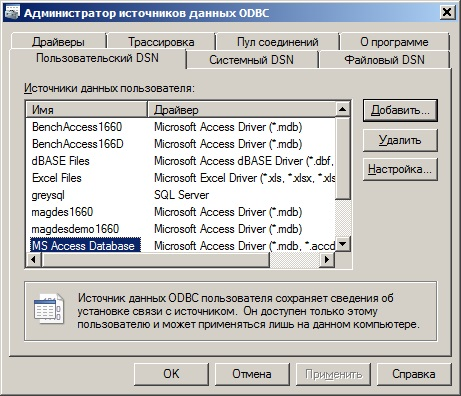
\includegraphics[width=0.5\linewidth]{bd_odbc_1.jpg}}
	\end{figure}
	
	\item Жмем \textit{<<Добавить>>} и выбираем драйвер \textit{<<Microsoft Access Driver (*.mdb, *accdb)>>}.
	
	\begin{figure}[H]
		\center{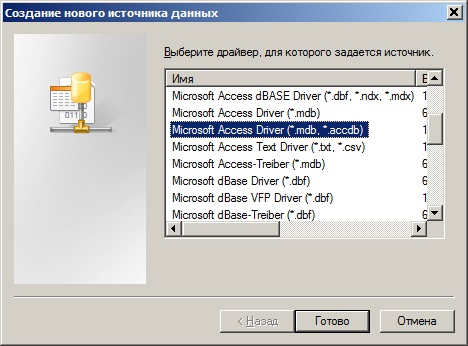
\includegraphics[width=0.5\linewidth]{bd_odbc_2.jpg}}
	\end{figure}
	
	\info{ Если данный пункт отсутствует, необходимо установить \textbf{Microsoft Access}.}
	
	\item Жмем \textit{<<Готово>>}, в~открывшейся форме выбираем необходимую \textbf{БД} и заполняем поля.
	
	\begin{figure}[H]
		\center{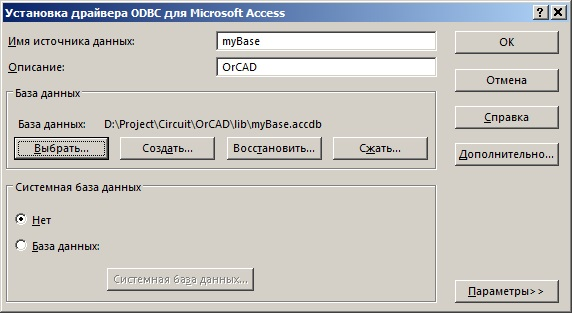
\includegraphics[width=0.5\linewidth]{bd_odbc_3.jpg}}
	\end{figure}
	
	\item Жмем \textit{<<OK>>} и проверяем что база появилась в списке.
\end{enumerate}



%%%------- Настройка multi-values полей
\subsubsection{Настройка multi-values полей} \label{sssec:bd_multi_value}

Начиная с версии \textbf{16.6}, каждое поле \textbf{БД} может являться \textbf{multi-values}, т.е. можно записывать несколько значений.

Для этого необходимо поместить в автозагрузку скриптов: \\
\textit{C:/SPB\_Data-Silent/cdssetup/OrCAD\_Capture/tclscripts/capAutoLoad} или \\
\textit{C:/Cadence/SPB\_16.6/tools/capture/tclscripts/capAutoLoad}), \\
файл \textit{*.tcl} со следующим содержимым:
\lstinputlisting[language=tcl]{OrCAD/CISRowColor.tcl}	% листинг файла

В примере выше, \textbf{multi-values} параметром объявляется \textit{<<Local Data>>}. Добавление других параметров осуществляется там же, например: 
\begin{center}
	\textit{SetCISMultiValuedField \{Datasheet\}}
\end{center}



%%%------- Подключение в CIS
\subsubsection{Подключение в CIS} \label{sssec:bd_setup_cis}

Подключение зарегистрированной в~системе \hyperlink{sssec:bd_install}{\textbf{БД}} происходит в~несколько шагов:
\begin{enumerate}
	\item Запустить \textbf{Design Entry CIS};
	\item Создать новый проект или открыть имеющийся;
	\item Перейти в окно \textit{<<Menu -> Options -> CIS Configuration\ldots>>};
		\begin{figure}[H]
			\center{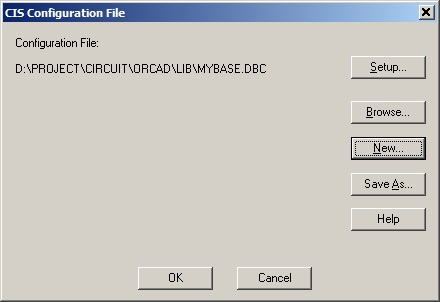
\includegraphics[width=0.6\linewidth]{bd_setup_1.jpg}}
		\end{figure}
	\item Перейти в окно создания нового подключения \textit{<<New\ldots>>};
	\item Выбрать из списка нужную базу;
	\item Выбрать нужные таблицы;
		\begin{figure}[H]
			\center{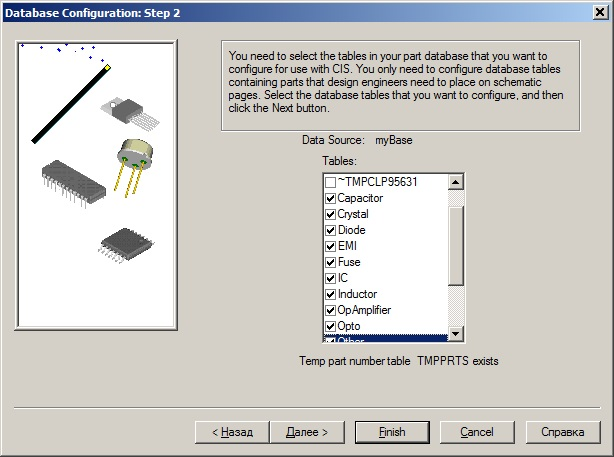
\includegraphics[width=0.6\linewidth]{bd_setup_2.jpg}}
		\end{figure}
	\item Выбрать соответствие между полями таблицы и параметрами \textbf{CIS}; 
		\begin{figure}[H]
			\center{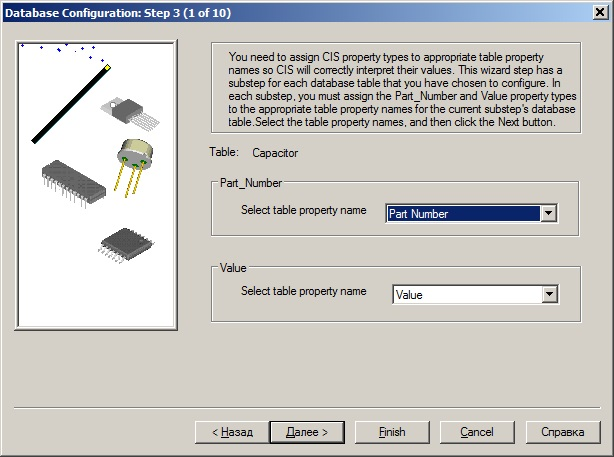
\includegraphics[width=0.6\linewidth]{bd_setup_3.jpg}}
		\end{figure}
		\info{Поля с одинаковыми именам заполняются автоматически.}
		\begin{figure}[H]
			\center{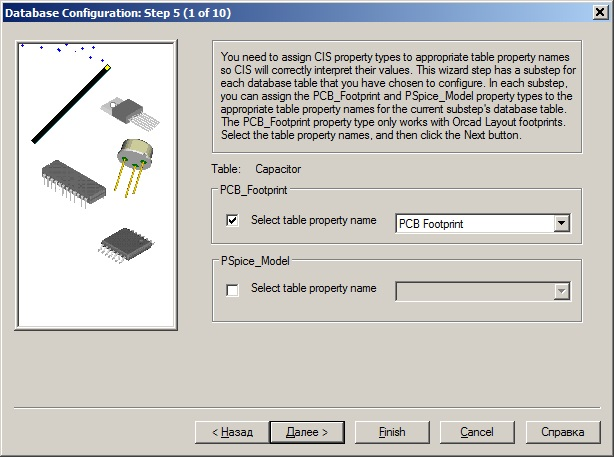
\includegraphics[width=0.6\linewidth]{bd_setup_4.jpg}}
		\end{figure}		
	\item Выбрать поля которые будут передаваться из БД в проект. Если \textbf{БД} заполнялась в соответствии с \hyperlink{sssec:bd_contet}{рекомендациями}, то как минимум должны быть отмечены: \textit{<<Value>>, <<PCB Footrpint>>, <<ALT\_SYMBOLS>>, <<NC>>, <<Description>>};
		\begin{figure}[H]
			\center{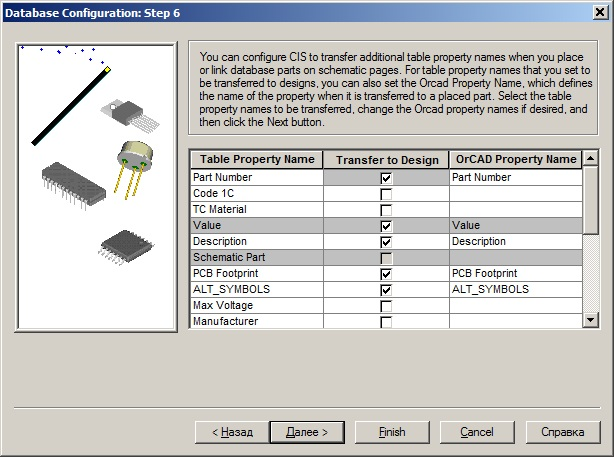
\includegraphics[width=0.6\linewidth]{bd_setup_5.jpg}}
		\end{figure}
	\item Если в дальнейшем планируется пользование \textbf{ICA}, то установить флаг \textit{<<ICA Properties>>}, иначе \textit{<<No ICA Properties>>};
		\begin{figure}[H]
			\center{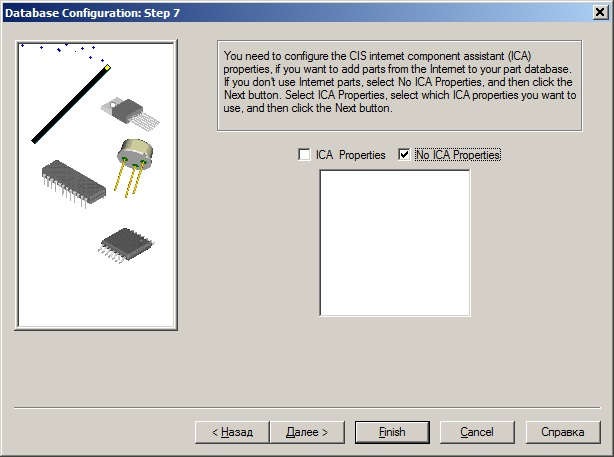
\includegraphics[width=0.6\linewidth]{bd_setup_6.jpg}}
		\end{figure}
	\item Выбрать какие параметры являются ссылками. Например: \textit{<<Datasheet>>} и \textit{<<Local Data>>};
		\begin{figure}[H]
			\center{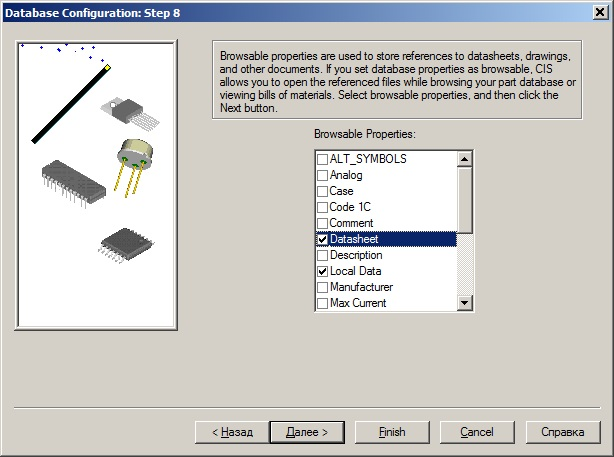
\includegraphics[width=0.6\linewidth]{bd_setup_7.jpg}}
		\end{figure}
	\item Выбрать параметры, которые будут видимы на схеме при установке элементов. Например: \textit{<<Part Number>>};
		\begin{figure}[H]
			\center{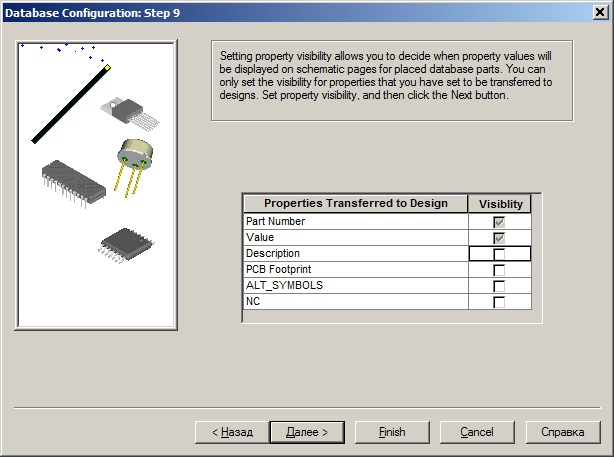
\includegraphics[width=0.6\linewidth]{bd_setup_8.jpg}}
		\end{figure}
	\item Выбрать ключевые поля
		\begin{figure}[H]
			\center{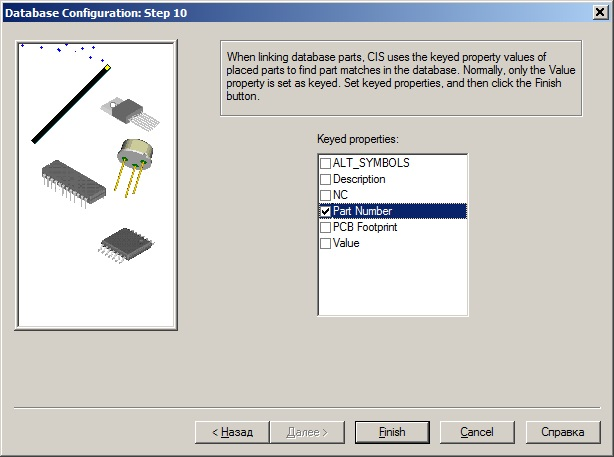
\includegraphics[width=0.6\linewidth]{bd_setup_9.jpg}}
		\end{figure}	
	\item В окне \textit{<<Configure Database>>} перейти на вкладку \textit{<<Administrative Preferences>>}. Снять флаги \textit{<<Allow Duplicate Part Numbers>>} и \textit{<<Assign Temportary Part Numbers Automatically>>}. В поле \textit{<<Delimiter for Multi-Values>>} ввести знак разделителя, который используется в \textbf{БД}. Если она заполнена согласно \hyperlink{sssec:bd_contet}{рекомендациям}, то это будет \textbf{запятая};
		\begin{figure}[H]
			\center{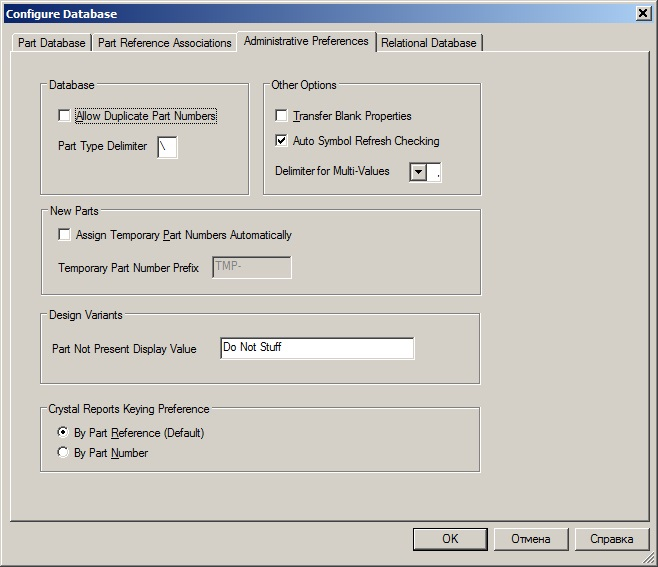
\includegraphics[width=0.6\linewidth]{bd_setup_10.jpg}}
		\end{figure}
	\item Во вкладке \textit{<<part Database>>} проверить настройки полей для каждой из таблиц и нажать \textit{<<OK>>}.
		\info{В дальнейшем вернуться в окно настроек \textit{<<Configure Database>>} можно так: \textit{<<Options -> CIS Configuration\ldots -> Setup>>}.}
		\begin{figure}[H]
			\center{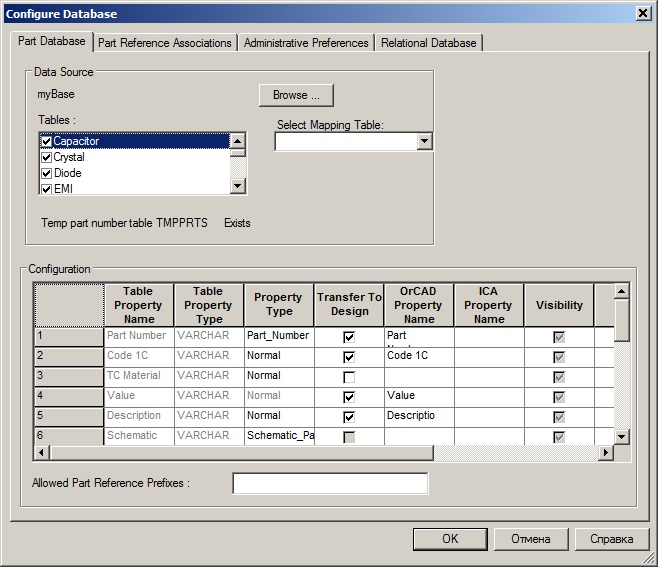
\includegraphics[width=0.6\linewidth]{bd_setup_11.jpg}}
		\end{figure}
	
\end{enumerate}



%%------- Создание символа УГО
\newpage
\subsection{Создание символа УГО} \label{ssec:create_symbol}

Пины \textit{<<Zero Length>>} обычно используются для силовых выводов, т.е. \textit{<<Power>>}.

%%%------- Стандартный способ
\subsubsection{Стандартный способ} \label{sssec:create_symbol_standart}

В окне проекта нажать \textbf{RMB} на нужной библиотеке и выбрать \textit{<<New Part>>}. Если необходим символ без привязки к физической реализации, вместо \textit{<<New Symbol>>} выбираем \textbf{<<New Symbol>>}, который позволяет определить следующие типы символов: \textit{<<Power>>, <<Off-Page Connector>>, <<Hierarchical Port>>, <<Title Block>> , <<Pin Shape>>}.

Переход между символами многосекционного УГО осуществляется при помощи \textit{<<Menu -> View -> Package>>} или кнопок \textbf{<<Ctrl+N>>} и \textbf{<<Ctrl+B>>}.

Таблицу настроек пинов можно вызвать из общего вида (\textit{<<Menu -> View -> Package>>}) \textit{<<Menu -> Edit -> Properties\ldots>>}. \textit{<<Pin Group>>} при этом обозначает эквивалентность выводов.
	\begin{figure}[H]
		\center{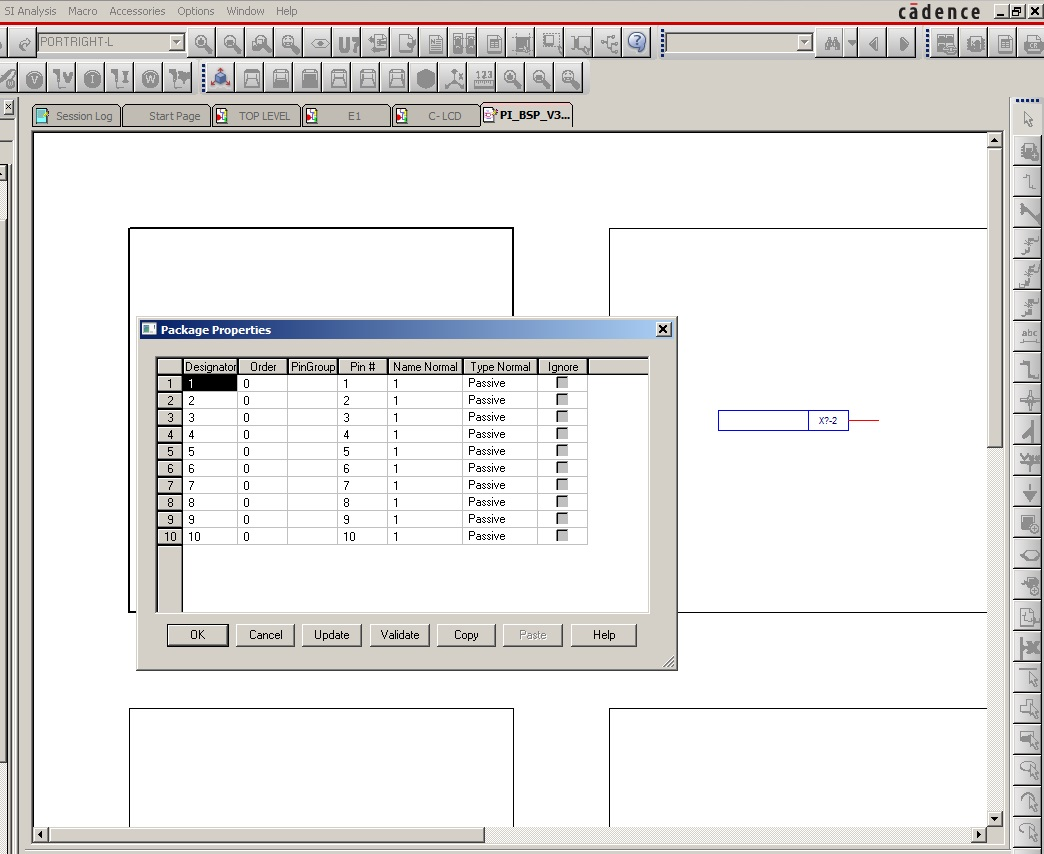
\includegraphics[width=0.6\linewidth]{create_symbol_1.jpg}}
	\end{figure}

%%%------- Табличный способ
\subsubsection{Табличный способ} \label{sssec:create_symbol_table}

В окне проекта нажать \textbf{RMB} на нужной библиотеке и выбрать \textit{<<New Part From Spreadsheet>>}.

Для изменения нескольких ячеек одновременно, надо удерживать \textbf{<<Shift>>}. 

Вернуться к таблице во время редактирования символа можно нажав \textbf{RMB} на элементе и выбрав \textit{<<Split Part>>}.
	\begin{figure}[H]
		\center{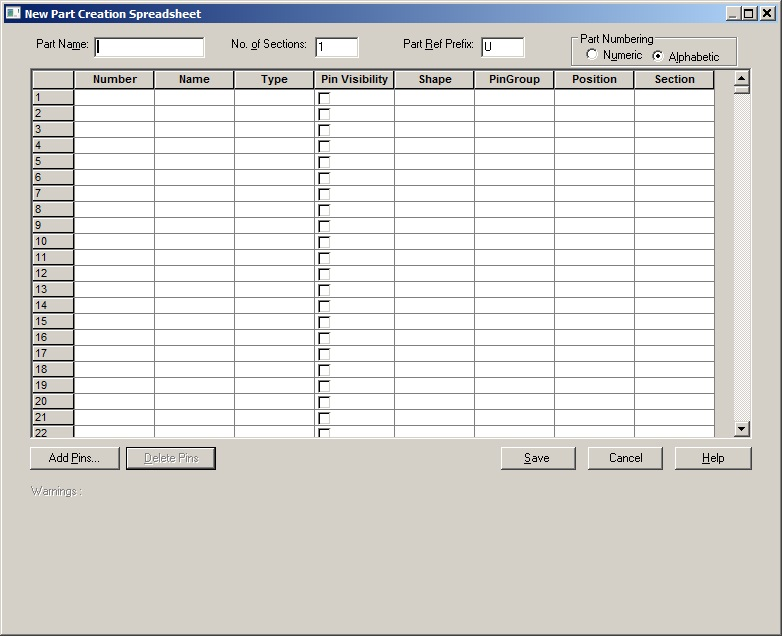
\includegraphics[width=0.6\linewidth]{create_symbol_2.jpg}}
	\end{figure}



%%%------- По данным из файла
\subsubsection{По данным из файла} \label{sssec:create_symbol_file}

При помощи данной опции можно создавать \textbf{УГО} по полученным из файла, созданным например для \textbf{ПЛИС} из проекта \textbf{Quartus}, данным.

В окне проекта перейти во вкладку \textit{<<Menu -> Tools -> Generate Part>>}. При первом создании установить флаг \textit{<<Create new part>>}, для обновления \textit{<<Update pins on existing part in library>>}.

	\begin{figure}[H]
		\center{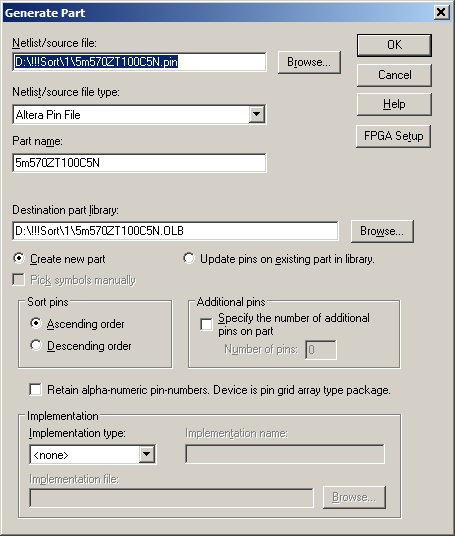
\includegraphics[width=0.6\linewidth]{create_symbol_3.jpg}}
	\end{figure}

При обновлении расположение выводов останется в соответствии с данными именами. 

Для удобства добавления дополнительных ножек, можно при создании символа зарезервировать несколько ножек в \textit{<<Additional pins>>}. Либо в последствии добавить на символ ножку с нужным именем и уже после этого переходить в \textit{<<Generate Part>>}. 

%%%------- По SPICE описанию
\subsubsection{По SPICE описанию} \label{sssec:create_symbol_spice}



%%-------
\newpage
\subsection{Вариантные исполнения} \label{ssec:variant_list}



%%%-------
\subsubsection{Передача в PCB Editor} \label{sssec:export_variant_list}

Передача вариантных исполнений из~схемного редактора в~редактор печатных плат, осуществляется в~несколько шагов:
\begin{enumerate}
	\item Запустить \textbf{Design Entry CIS};
	
	\item Перейти в~окно \textit{Part Manager};
	
	\item Сформировать список вариантных исполнений \textit{<<Menu -> Tools -> Export Variant List>>}; 
	
	\item Запустить \textbf{PCB Editor};
	
	\item Перейти в~окно \textit{<<Menu -> Manufacture -> Variants -> Create Assembly Drawing...>>};
	
	\item Выбрать нужные настройки и вариант исполнения.
	
		\begin{figure}[H]
			\center{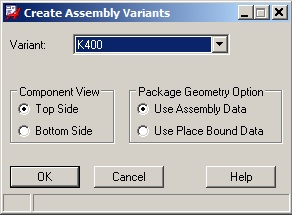
\includegraphics{create_assembly_variants.jpg}}
%			\caption{Окно вариантного исполнения} 
%			\label{fig:create_assembly_variants}
		\end{figure}	
	
\end{enumerate}

После этих действий появится новый подкласс в~классе \textit{Manufacture}. Для настроек установленных выше это будет \textit{<<Manufacture/K400\_Top>>}.


%%-------
\newpage
\subsection{Надстройки} \label{ssec:variant_list} \label{ssec:cis_plugin}



%%%-------
\subsubsection{Подключение} \label{sssec:cis_plugin_setup}

Для автоматической загрузки, необходимо разместить скачанные \textbf{tcl} скрипты в~папку \textit{<<\%CDS\_SITE\%/OrCAD\_Capture/tclscripts/capAutoLoad/>>}, либо создать там отдельную папку.

Для загрузки в ручную, необходимо разместить скачанные \textbf{tcl} скрипты в~папку \textit{<<\%CDS\_SITE\%/OrCAD\_Capture/tclscripts/>>}, либо создать там отдельную папку.


